% !TEX root = ../main.tex
\subsection{CLAS12} \label{ssec::clas12}
    \begin{figure}[b!]
        \centering\frame{
        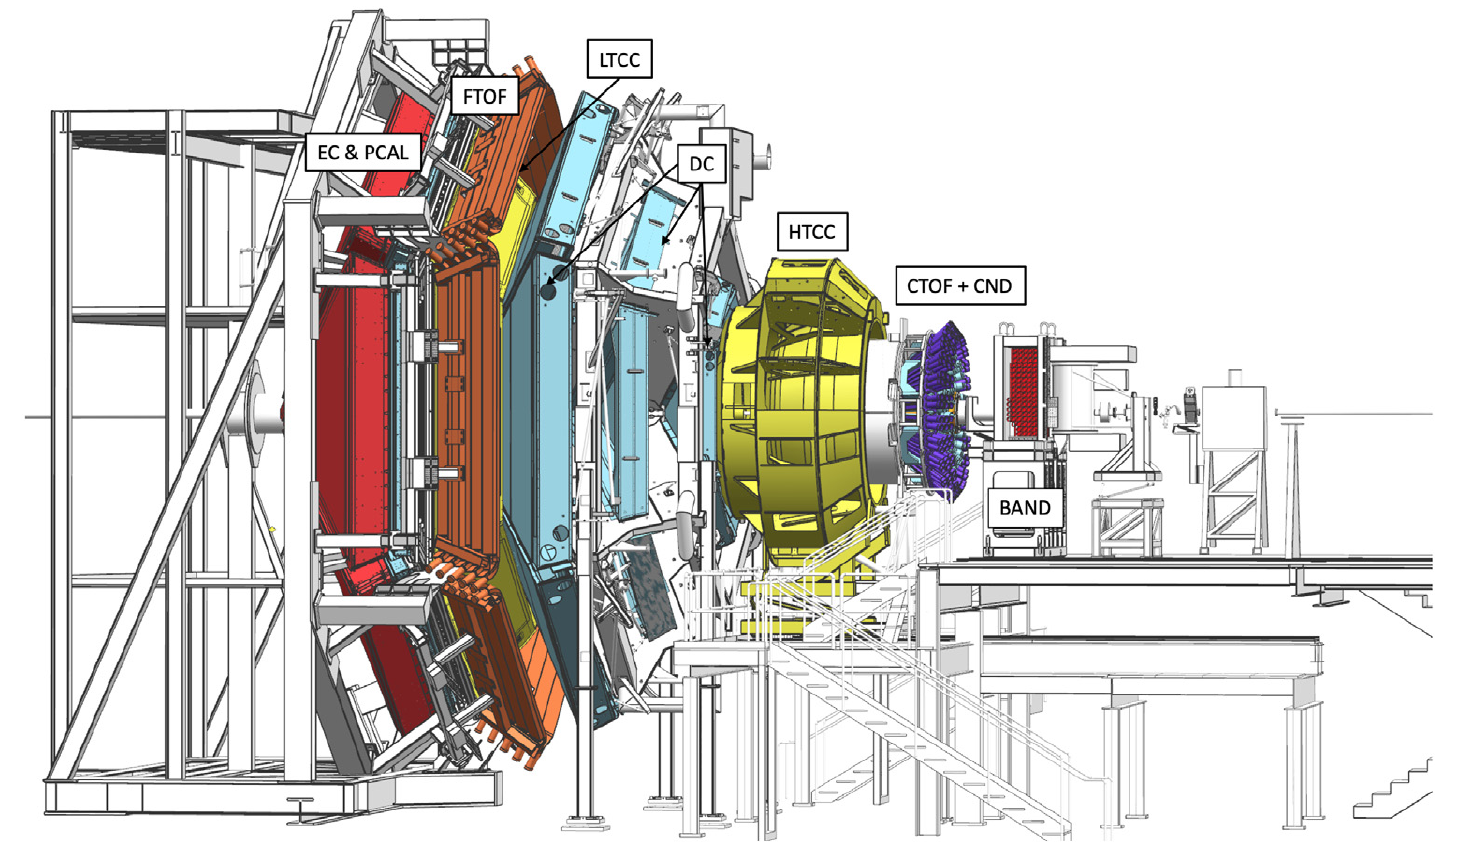
\includegraphics[width=\textwidth]{11experiment/img/20clas12_diagram.png}}
        \caption[CLAS12.]{The CLAS12 detector in the Hall B beamline.
        The electron beam enters from the right and impinges on the target located in the center of the solenoid magnet shown at the right (upstream) end of CLAS12.
        The FD consists of the High Threshold Cherenkov Counter (HTCC) (yellow), the torus magnet (grey), the DC tracking system (light blue), and another set of Cherenkov counters (hidden), time-of-flight scintillation counters (brown), and Electromagnetic Calorimeters (ECs) (red).
        Between the HTCC and the torus, the Forward Tagger (FT) is installed.
        The CD consists of the Silicon Vertex Tracker (SVT) (hidden), which is surrounded by a Barrel Micromesh Tracker (BMT) (hidden), the Central Time-of-Flight (FTOF) system, and the Central Neutron Detector (CND) (blue).
        At the upstream end, a Back Angle Neutron Detector (BAND) (red) is installed.
        Source: \hyperlink{https://www.jlab.org/physics/hall-b/clas12}{CLAS12 wiki}.}
        \label{fig::clas12_diagram}
    \end{figure}

    The main detector in Hall B is CLAS12, and is used to study electro-induced nuclear and hadronic reactions.
    The spectrometer provides efficient detection of charged and neutral particles over a large fraction of the full solid angle.

    CLAS12 is based on two superconducting magnets: a solenoid magnet and a $5$ T torus magnet.
    The detector is separated into two detectors, the Forward Detector (FD) and the Central Detector (CD).
    FD, aided by the torus magnet, covers the forward polar range from $5\degree$ up to $35\degree$.
    CD, aided in turn by the solenoid magnet, covers the polar angles from $35\degree$ to $125\degree$.
    Both detectors have full azimuthal coverage.

    Trajectory reconstruction is done in the forward direction using Drift Chambers (DC) with a momentum resolution of $< 1\%$.
    In turn, in the central detector it is done by a vertex tracker, resulting in a momentum resolution of $< 3\%$.
    Cherenkov counters, time-of-flight scintillators, and electromagnetic calorimeters are used for particle identification.
    Fast triggering and high data-acquisition rates allow operation at a luminosity of $10^{35} \text{cm}^{-2}\text{s}^{-1}$ \cite{burkert2020}.
    
    A diagram of CLAS12 detailing the position of every detector inside is provided in Figure \ref{fig::clas12_diagram}

    % !TEX root = ../main.tex
\subsubsection{Forward Detector} \label{sssec::forwarddetector}

% --+ HTCC +--------------------------------------------------------------------
\paragraph{High Threshold Cherenkov Counter (HTCC)}
    \begin{wrapfigure}{l}{0.50\textwidth}
        \centering\frame{
        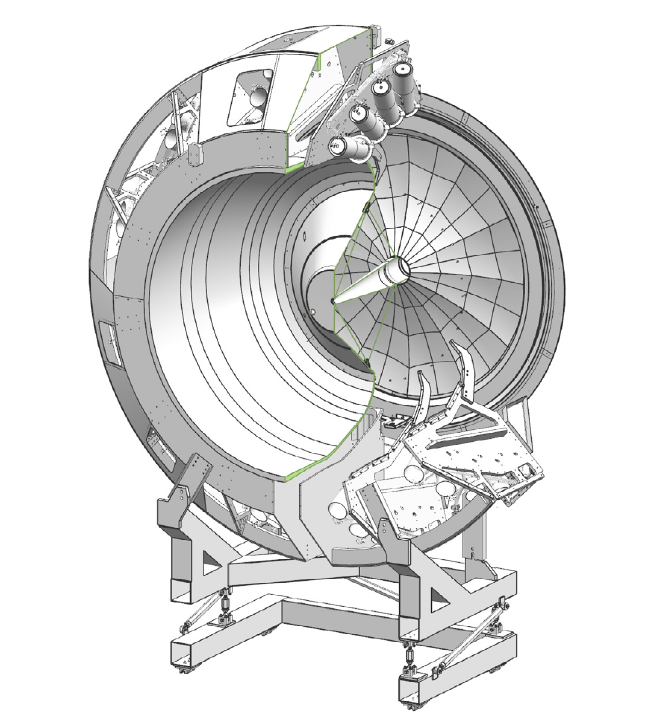
\includegraphics[width=\linewidth]{11experiment/img/21htcc.png}}
        \caption[HTCC]{Render of the High Threshold Cherenkov Counter.
        The container spans a diameter of about 4.5 m. The mirror is seen at the downstream end to the right.
        The PMTs are mounted in 12 sectors and in groups of 4 at the outer perimeter of the container.
        Light collection uses additional Winston cones and 5-in PMTs with quartz windows.}
        \label{fig::htcc}
    \end{wrapfigure}

    The HTCC is the main detector to separate electrons and positrons with momenta below 4.9 GeV from other charged particles.
    The detector has full azimuthal coverage and spans from $5\degree$ to $35\degree$ in polar angle.
    It has no blind areas in its complete solid angle coverage.
    The detector is located downstream of the target, fitted in between magnets, upstream of the forward tracking detectors.

    The HTCC system is mainly used for electron/positron identification, and thus it provides high rejection of charged pions and low background noise for reliable identification of scattered electrons in a dense electromagnetic background environment.
    The HTCC is a single unit operated in dry CO2 gas at 1 atm pressure.
    It is constructed using a multi-focal mirror of 48 elliptical mirror facets that focuses the Cherenkov light on 48 PhotoMultiplier Tubes (PMTs), each with a quartz window of 125 mm diameter.
    The PMTs are located in a magnetic field of up to $3.5\cdot 10^{-3}$ T oriented along the phototube axes and are surrounded along their lengths by a multi-layer magnetic shield with active compensation coils.

    In order to minimize multiple scattering in the HTCC detector materials and to limit its impact on the momentum analysis of charged tracks in the torus field, the HTCC mirror system is constructed using a backing structure of low-density composite material.
    As the detector is located in front of the momentum analysing torus magnet, all materials but the radiator gas in the path of the charged particles had to be kept to a minimum.
    In the actual detector, the density of the solid material seen by charged particles passing through the HTCC volume is $135 ~\text{mg}/\text{cm}^2$.
    The HTCC is also used to generate a fast signal to be used as a trigger for scattered electrons.
    The HTCC operates in conjunction with energy deposited in the electromagnetic calorimeters to identify electrons of specific energies \cite{sharabian2020}.
    A cut view of HTCC can be seen in Figure \ref{fig::htcc}.

% --+ DC +----------------------------------------------------------------------
\paragraph{Drift Chambers (DC)}
    \begin{wrapfigure}{r}{0.50\textwidth}
        \centering\frame{
        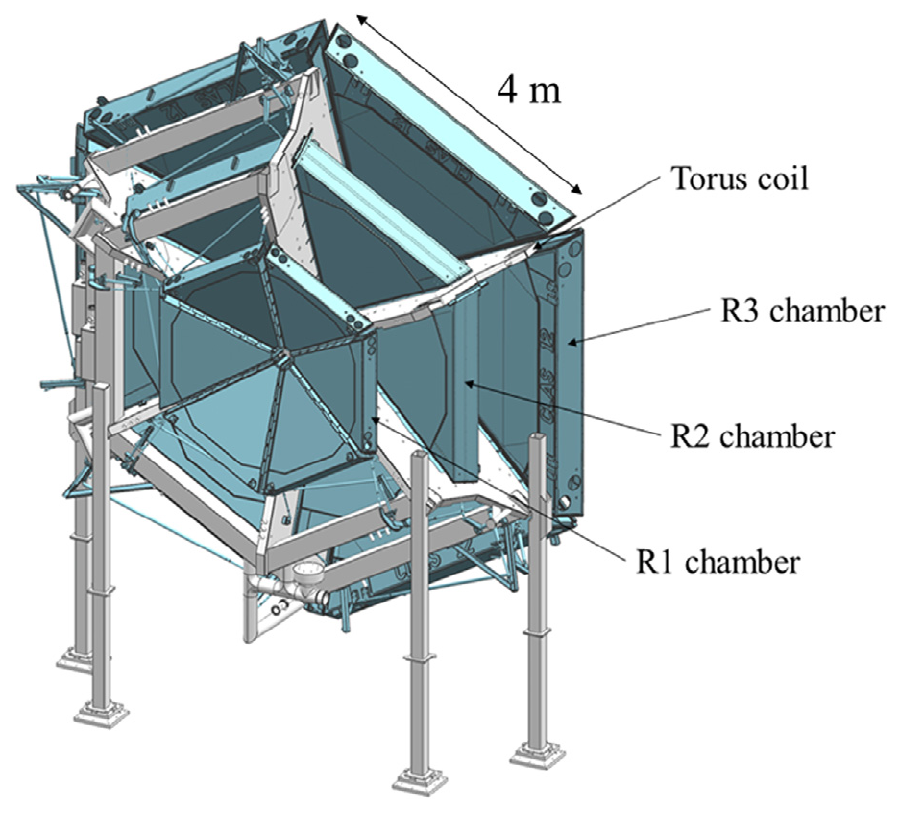
\includegraphics[width=\linewidth]{11experiment/img/21dc.png}}
        \caption[DC]{Drift Chambers render.
        Each of the DC regions are denoted as R1, R2, and R3 in the figure.}
        \label{fig::dc}
    \end{wrapfigure}

    The six coils of the torus magnet act as support for the forward tracking system, which consists of three independent drift chambers in each of the six sectors of the torus magnet.
    Each of the six DC sectors has a total of 36 layers with 112 sense wires each, arranged in three regions of twelve layers each.
    In each of the six torus sectors, the drift chambers are arranged identically.
    The arrangement of the DC around the torus coil can be seen in Figure \ref{fig::dc}

    As can be seen on the figure, the first region is located at the entrance to the torus magnetic field region.
    Then, the second is inside the magnet, where the magnetic field is close to its maximum.
    The third is located in a low magnetic field space, just downstream of the torus magnet.
    This arrangement provides independent and redundant tracking in each of the six torus sectors.

    Each of the three regions consists of six ``superlayers'', each of which contains two layers.
    One layer has wires strung at a stereo angle of $+6\degree$ while the second one of $-6\degree$, both with respect to the sector midplane.
    This stereo view enables excellent resolution in the polar angle ($\Delta\theta < 2 ~\text{mrad}$), and good resolution in the azimuthal scattering angle ($\Delta\phi < 2 ~\text{mrad}$).

    The DC can detect ionising particles with momenta above $200 ~\text{MeV}/\text{c}$, with a $\Delta p/p$ lesser than $0.5\%$.
    This offers a track momentum resolution of $3$ to $5\%$ \cite{mestayer2020}.

% --+ LTCC +--------------------------------------------------------------------
\paragraph{Low Threshold Cherenkov Counter (LTCC)}
    The LTCC system is used for charged pion and kaon detection at momenta between $3.5$ and $9 ~\text{GeV}$.
    The LTCC system consists of boxes shaped like truncated pyramids.
    Four of the six sectors of CLAS12 are equipped with one LTCC box.
    Each LTCC box contains 108 lightweight mirrors with composite backing structures, 36 Winston light-collecting cones, 36 125-mm diameter PMTs, and 36 magnetic shields.
    The LTCC boxes are filled with heavy C4 F10 radiator gas.

    \begin{wrapfigure}{l}{0.50\textwidth}
        \centering\frame{
        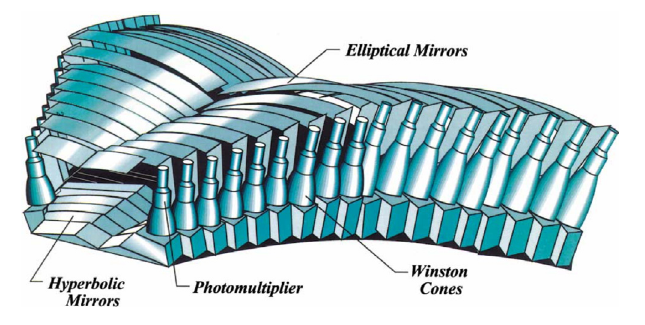
\includegraphics[width=\linewidth]{11experiment/img/21ltcc.png}}
        \caption[LTCC Mirror System]{Layout and components of the optical mirror system within each LTCC box from the design model.}
        \label{fig::ltcc}
    \end{wrapfigure}

    The LTCC was a detector used in CLAS, which as part of the 12 GeV upgrade was refurbished to provide higher efficiency for charged pion and kaon detection.
    This was done by increasing the volume of the radiator gas, refurbishing the elliptical and hyperbolic mirrors with new coatings, and improving the sensitivity of the PMTs to Cherenkov light.
    The sensitivity improvement was achieved by coating their entrance windows with wavelength shifting material that absorbs ultraviolet (UV) light at wavelength below $300 ~\text{nm}$ and re-emits two back-to-back photons at larger wavelength \cite{ungaro2020}.
    A drawing from the design model of the LTCC can be seen in Figure \ref{fig::ltcc}.

% --+ FTOF +--------------------------------------------------------------------
\paragraph{Forward Time-of-Flight (FTOF)}
    \begin{wrapfigure}{r}{0.50\textwidth}
        \centering\frame{
        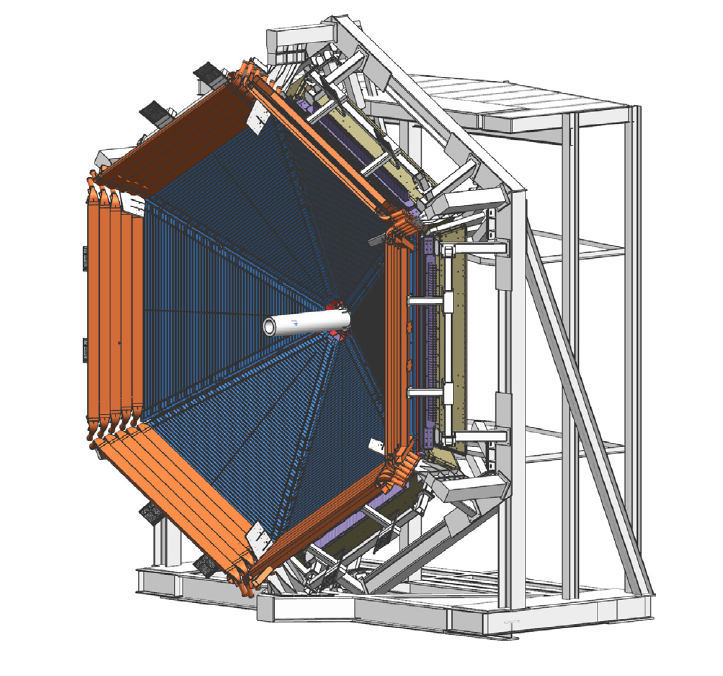
\includegraphics[width=\linewidth]{11experiment/img/21ftof.png}}
        \caption[FTOF]{Render of the Forward Carriage with the FTOF system showing the panel-1b counters on the inside (dark blue), and the panel-2 counters on the outside (bronze).
        The panel-1a counters are located immediately downstream of the panel-1b counters and are not visible in the render.
        Part of the PCAL is visible downstream of the FTOF panels.}
        \label{fig::ftof}
    \end{wrapfigure}

    The FTOF system is used to measure the TOF of charged particles emerging from the target during beam operation.
    It includes six sectors of plastic scintillators with double-sided PMT readout.
    Each sector consists of three arrays of counters separated in panels, with panel-1a having 23 counters, panel-1b 62 counters, and panel-2 5 counters.
    The system is required to get excellent timing resolution required for particle identification and good segmentation to get flexible triggering options.

    The detectors span a range in polar angle from $5\degree$ to $45\degree$, covering $50\%$ in the azimuth at $5\degree$ and $90\%$ at $45\degree$.
    The lengths of the counters range from $32.3 ~\text{cm}$ to $376.1 ~\text{cm}$ in panel 1a, from $17.3 ~\text{cm}$ to $407.9 ~\text{cm}$ in panel-1b, and from $371.3 ~\text{cm}$ to $426.2 ~\text{cm}$ in panel-2.
    The average timing resolution in panel-1a is $125 ~\text{ps}$, $85 ~\text{ps}$ in panel-1b, and $155 ~\text{ps}$ in panel-2 \cite{carman2020ftof}.
    A render of the detector can be seen in Figure \ref{fig::ftof}.

% --+ RICH +--------------------------------------------------------------------
\paragraph{Ring Imaging Cherenkov Detector (RICH)}
    For momenta greater than 3 GeV, the TOF resolution of FTOF is not sufficient to separate kaons from pions.
    For that puspose, an additional RICH detector was built and incorporated into one of the CLAS12 sectors to replace the corresponding LTCC sector.
    The RICH detector is designed to improve CLAS12 particle identification in the momentum range $3 - 8 ~\text{GeV}$.
    The detector incorporates aerogel radiators, visible light photon detectors, and a focusing mirror system that is used to reduce the detection area instrumented by photon detectors to $1 ~\text{m}^2$.

    Multi-anode PhotoMultiplier Tubes (MaPMTs) provide the required spatial resolution and match the aerogel Cherenkov light spectrum in the visible and near-UV region.
    For forward scattered particles up to $13\degree$ with momenta $3 - 8 ~\text{GeV}$, a proximity imaging method with thin ($2 ~\text{cm}$) aerogel and direct Cherenkov light detection is used.
    For larger incident particle angles between $13\degree$ and $25\degree$ and momenta of $3 - 6 ~\text{GeV}$, the Cherenkov light is produced by a thicker aerogel layer of $6 ~\text{cm}$, focused by a spherical mirror, and undergoes two further passes through the thin radiator material and a reflection from planar mirrors before detection \cite{contalbrigo2020}.

% --+ ECAL +--------------------------------------------------------------------
\paragraph{Electromagnetic Calorimeters (ECAL)}
    The CLAS12 detector package uses the existing electromagnetic calorimeter (EC) of the CLAS detector, but adds to it a new pre-shower calorimeter (PCAL), which is installed upstream of the EC.
    Together, the PCAL and EC are referred to as the ECAL.
    The calorimeters in CLAS12 are used primarily for the identification and kinematical reconstruction of electrons, photons, and neutrons.

    The PCAL and EC are both sampling calorimeters consisting of six modules.
    Along the direction from the target, the EC consists of two parts, read out separately, called EC-inner (ECIN) and EC-outer (ECOU).
    They provide longitudinal sampling of electromagnetic showers, as well as of hadronic interactions to improve particle identification.
    Each module has a triangular shape with 54 (15/15/24, PCAL/ECIN/ECOU) layers of 1-cm-thick scintillators segmented into 4.5/10-cm (PCAL/EC) wide strips fitted between 2.2-mm-thick lead sheets.
    The total thickness corresponds to approximately 20.5 radiation lengths.
    Scintillator layers are grouped into three readout views with 5/5/8 PCAL/ECIN/ECOU layers per view, providing spatial resolutions of less than $2 ~\text{cm}$ for energy clusters.
    The light from each scintillator readout group is routed to the PMTs via flexible optical fibres \cite{asryan2020}.

% --+ FT +----------------------------------------------------------------------
\paragraph{Forward Tagger (FT)}
    The FT extends the capabilities of CLAS12 to detect electrons and photons at the very forward polar angles from $2.5\degree$ to $4.5\degree$.
    The detection of forward-going scattered electrons allows for electroproduction experiments at very low photon virtuality $Q^2$, providing an energy-tagged, linearly polarized, high-intensity, quasi-real photon beam.
    This configuration enables execution of an extensive hadron spectroscopy program.

    \begin{wrapfigure}{l}{0.50\textwidth}
        \centering\frame{
        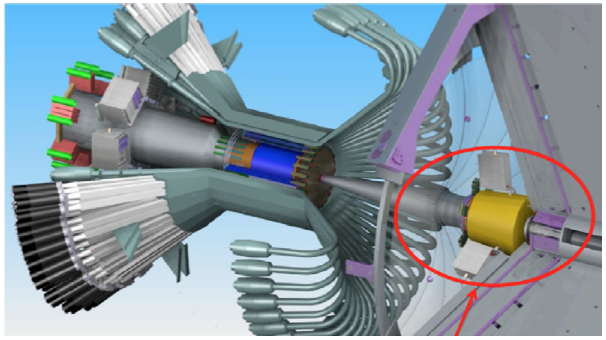
\includegraphics[width=\linewidth]{11experiment/img/21ft.png}}
        \caption[FT]{The Forward Tagger system circled downstream of the CD in front of the torus magnet warm bore entrance.}
        \label{fig::ft}
    \end{wrapfigure}

    The FT consists of a calorimeter (FTCal), a micro-strip gas tracker (FTTrk), and a hodoscope (FTHodo).
    The FTCal with 332 lead-tungstate ($\text{PbWO}_4$) crystals is used to identify electrons, measure the electromagnetic shower energy, and provide a fast trigger signal.
    The FTTrk in front of it measures the charged particle scattering angles.
    The scintillator FTHodo aids in separating electrons and high-energy photons.

    During beam operations, a tungsten shielding pipe of conical shape is installed in front of the FT to absorb M\o ller electrons and low-energy photons produced by beam interactions with the target and downstream materials.
    This shield protects both the FT and the Forward Detectors from electromagnetic background.
    The cone angle is $2.5\degree$, such that it is compatible with the FT acceptance.
    In this configuration, known as ``FT-ON'', the FT can be used to detect both electrons and photons, extending the detection capabilities of CLAS12.

    \begin{wrapfigure}{r}{0.50\textwidth}
        \centering\frame{
        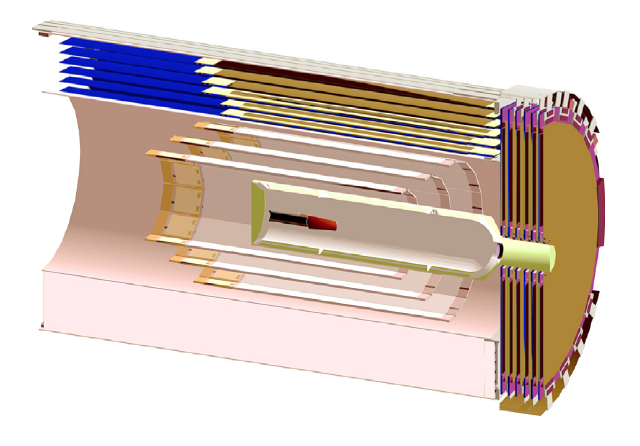
\includegraphics[width=\linewidth]{11experiment/img/22cvt.png}}
        \caption[CVT]{Render of the Central Vertex Tracker.
        From the inside, the figure shows the target cell and vacuum chamber, the three double layers of the SVT, followed by the six layers of the BMT.
        The beam enters from the left.
        The six FMT layers are shown at the downstream end at the right.}
        \label{fig::cvt}
    \end{wrapfigure}

    Alternatively, when the FT is not needed for the physics program, the FT detectors are turned off and additional shielding elements are installed in front of the FT covering up to $4.5\degree$ to reduce the background in the DC R1 chambers.
    This configuration, known as ``FT-Off'', reduces the accidental background by one-third at the same beam conditions, which allows for higher luminosity data taking with CLAS12 \cite{acker2020ft}.
    A render of the CD with the FT circled can be seen in Figure \ref{fig::ft}.

    % !TEX root = ../main.tex
\subsubsection{Central Detector} \label{sssec::centraldetector}
    Particles scattered from the target at polar angles in the range from $35\degree$ to $125\degree$ are detected in the CD with its own particle identification and tracking detectors.
    Charged particles are tracked in the Central Vertex Tracker (CVT) and detected in the Central Time-of-Flight (CTOF) detector with full coverage in azimuthal angle.
    Neutron detection is provided by the Central Neutron Detector (CND) located radially outside of the CVT and the CTOF.

% --+ CVT +---------------------------------------------------------------------
\paragraph{Central Vertex Tracker (CVT)}
    The CVT system is a part of the CD and is used to measure the momentum and to determine the vertex of charged particles scattered from the target.
    The tracker lies inside the solenoid magnet, as can be seen in Figure \ref{fig::cvt}.
    CVT consists of two separate detectors, a Silicon Vertex Tracker (SVT) and a
    Barrel MicroMegas Tracker (BMT).

    The SVT system includes three regions with 10, 14, and 18 double-sided modules of silicon sensors instrumented with a digital ASIC readout.
    The readout pitch is \SI{156}{\micro\metre}, and the total number of channels is 21,504 \cite{antonioli2020}.

    The BMT contains three layers of strips along the beamline and three layers of circular readout strips around the beamline, with a total number of 15,000 readout elements.
    The BMT provides important improvements in momentum resolution and in tracking efficiency.
    Each layer is arranged azimuthally in three segments of $120\degree$ azimuthal coverage each.
    The system operates at the full design luminosity of $10^{35} \text{cm}^{-2}\text{s}^{-1}$ \cite{acker2020mvt}.

    Another component of the CVT is the Forward MicroMegas Tracker (FMT), which consists of six layers with 6144 readout elements.
    It is integrated mechanically with the CVT to provide a compact tracking system, but covers the polar angle range from $5\degree$ to $35\degree$ and provides improved vertex reconstruction for forward-scattered charged particles \cite{acker2020mvt}.
    The FMT working principle and geometry are discussed in detail in Section \ref{sec::fmtalignmentandreconstruction}.

% --+ CTOF +--------------------------------------------------------------------
\paragraph{Central Time-of-Flight}
    \begin{wrapfigure}{r}{0.49\textwidth}
        \centering\frame{
        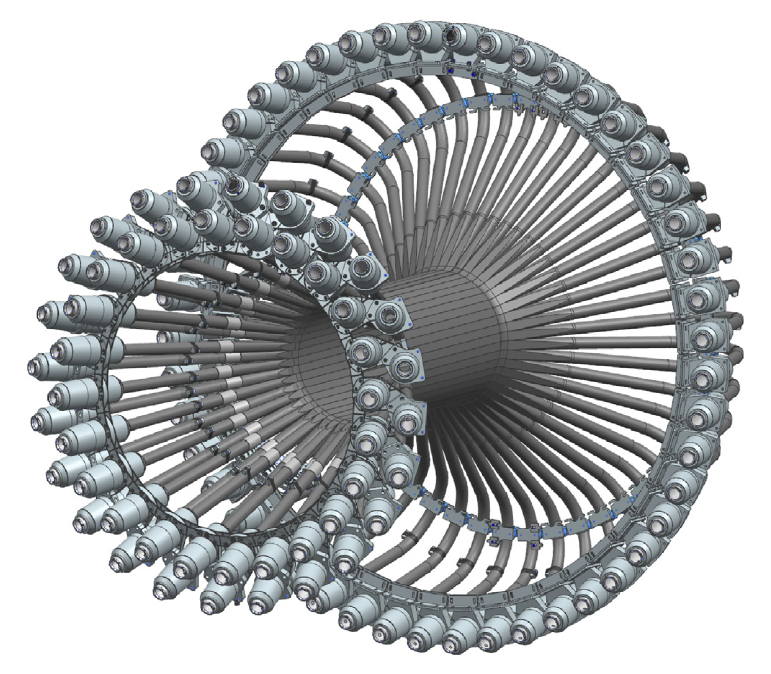
\includegraphics[width=\linewidth]{11experiment/img/22ctof.png}}
        \caption[Central Time-of-Flight]{Render of the Central Time-of-Flight.
        The render shows CTOF's 48 scintillator bars outfitted with light guides, PMTs, and magnetic shields at both ends of each counter.}
        \label{fig::ctof}
    \end{wrapfigure}

    The CTOF system is used for the identification of charged particles emerging from the target via TOF measurements in the momentum range from $0.3$ to about $1.25 ~\text{GeV}$.
    The CTOF includes 48 plastic scintillators with double-sided PMT readout via, respectively, 1.0-m-long upstream and 1.6-m-long downstream focusing light guides.
    The array of counters forms a hermetic barrel around the target and the CVT.
    The barrel is aligned with the beam axis inside the 5 T solenoid magnet.
    The PMTs are placed in a region of 0.1 T fringe field of the solenoid and enclosed within a triple layer dynamical magnetic shield that provides less than 0.2 G internal field near the PMT photocathode.
    The CTOF system is designed to provide time resolution of 80 ps for charged particle identification in the CLAS12 CD \cite{carman2020ctof}.
    A render of CTOF can be seen in figure \ref{fig::ctof}.

% --+ CND +---------------------------------------------------------------------
\paragraph{Central Neutron Detector (CND)}
    The CLAS12 CD is also equipped with the CND positioned radially outward of the CTOF.
    It allows the detection of neutrons in the momentum range from $0.2$ to $1.0 \text{GeV}$ by measurement of their TOF from the target and the energy deposition in the scintillator layers.
    The detector is made of three layers of scintillator paddles (48 paddles per layer), coupled two-by-two at the downstream end with semi-circular light guides.
    The signal is read out at the upstream end by PMTs placed outside of the high magnetic field region of the solenoid.
    The scintillators are connected to 1-m-long bent light guides \cite{chatagnon2020}.

% --+ BAND +--------------------------------------------------------------------
\paragraph{Back Angle Neutron Detector (BAND)}
    Neutron detection at back angles is accomplished with the BAND, which is positioned 3 metres upstream of the target.
    It detects backward neutrons with momenta between $0.25$ and $0.7$ GeV.
    The detector consists of 18 horizontal rows and five layers of scintillator bars with PMT readout on each end to measure TOF from the target.
    There is an additional $1 \text{cm}$ scintillation layer for vetoing charged particles.
    BAND covers a polar angle range from $155\degree$ to $175\degree$ with a design neutron detection efficiency of $35\%$ and a momentum resolution of about $1.5\%$ \cite{segarra2020}.

    % !TEX root = ../main.tex
\subsubsection{Offline Reconstruction} \label{sssec::offlinereconstruction}
    CLAS12 reconstruction and analysis relies on a data-stream processing framework called CLARA.
    CLARA provides a service-oriented architecture in which to build software applications composed of micro-services, linked together by data-stream pipes.
    The service-oriented framework allows for each engine to be encapsulated, helping guarantee a long lifetime and code modularity \cite{gyurgyan2016}.

    A service receives input data, processes it, and produces output data, where the I/O is organised into tabular structures called ``banks'' whose structure is configured by the specific service developer.
    A service reacts to an input data stream, processes it, and passes processed data to the next service in the data-flow path.
    As a result, the CLAS12 data processing application is versatile and flexible, since the application building blocks can be improved individually and replaced with no need for structural changes in the framework.
    % The CLAS12 services are extensions of an abstract reconstruction engine, which includes common components such as initialisation and event processing methods.
    % This approach reduces and simplifies the development of an individual micro-service and enforces a common structure.

    Data reader services access the detector decoded data stored in banks.
    Each entry for the decoded detector hits is a row in a bank.
    A row includes detector element identifiers (sector, layer, component, and order), and digitised detector data, such as signal charge, amplitude, time, or pedestal, depending on the specific system.
    Similar bank structures are created at the decoding stage for the various quantities needed for event reconstruction, such as hits, clusters, tracks, etc.
    The services that implement the reconstruction algorithms pertaining to the CLAS12 subsystems fill these banks, which are subsequently appended and written out to a file by a data-persistence service.

    The services running the reconstruction algorithms access the various banks as input and produce output banks needed for the subsequent algorithms in the reconstruction chain.
    The order in which the services are chained reflects the overall CLAS12 event reconstruction sequence and subsystem dependencies.
    First, charged particle tracks are reconstructed in both the Central and Forward Detector tracking systems based on the position of the recorded hits in the different detectors (i.e. using strip positions or wire locations).
    This procedure is referred to as ``hit-based'' tracking.

    In parallel, hits recorded in the other detectors are processed to reconstruct the energy and time of the associated particle interaction.
    These are matched to the reconstructed tracks by the Event Builder (EB) service, based on hit
    position and time information.
    Unmatched hits are retained as neutral particle candidates.
    At this stage, the EB can reconstruct the event ``start time'', or the time of the interaction between the beam and target, and identify the reconstructed particles.
    Once the event start time is determined, a second iteration of forward tracking can be performed to implement the so-called ``time-based'' tracking, which also incorporates the drift times in the Drift Chambers \cite{ziegler2020}.

    An overview of the reconstruction application service composition detailing these dependencies is shown in Figure \ref{fig::recon_chain}.

    \begin{figure}[t]
        \centering\frame{
        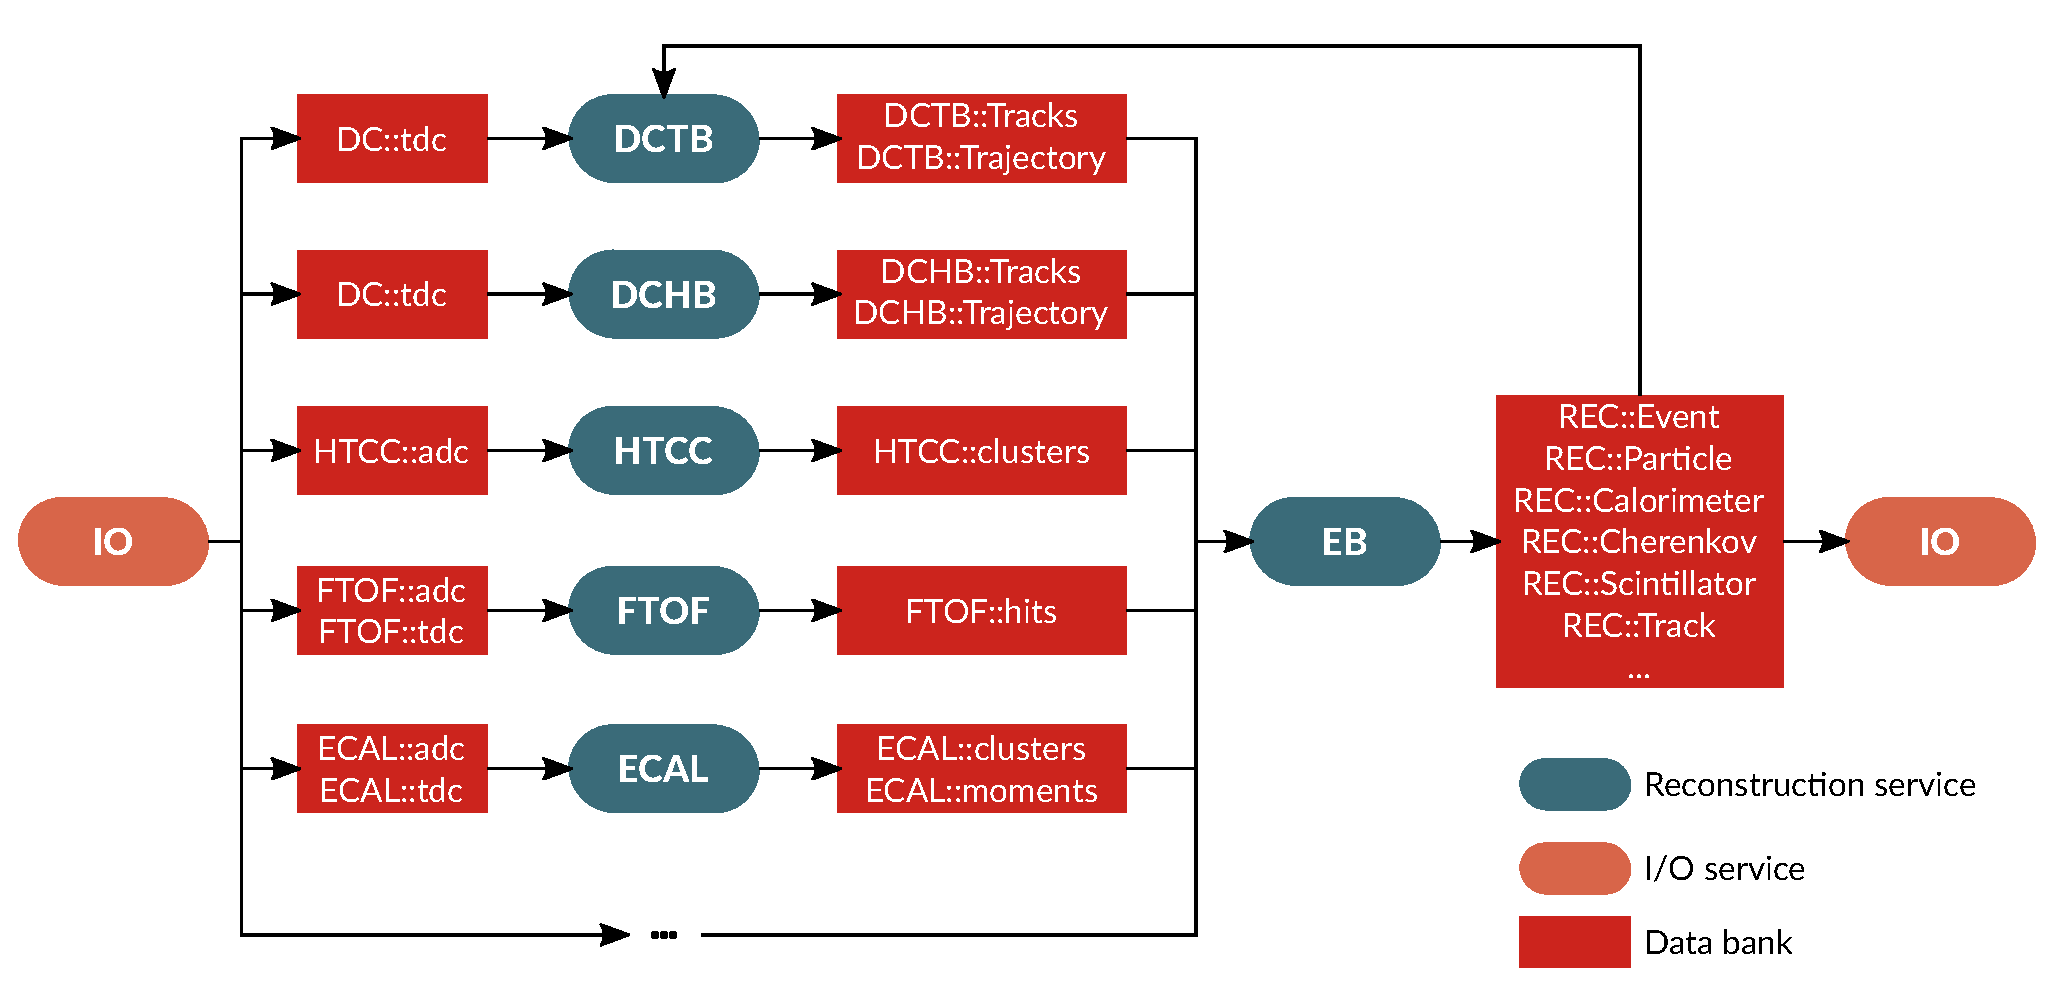
\includegraphics[width=\textwidth]{11experiment/img/23recon_chain.pdf}}
        \caption[CLAS12 Reconstruction Chain.]{Graphical representation of the CLAS12 interdependencies between services and banks.
        The I/O service reads events from the input file and distributes them to the reconstruction services chain for processing.
        Each service reads the relevant banks, applies the reconstruction algorithm, and provides output banks that are passed to the next service in the chain.
        The Event Builder (EB) service is executed as last in the chain; it collects the relevant banks from all CLAS12 subsystems services and produces event, particle, and detector response banks that are written to the output file.}
        \label{fig::recon_chain}
    \end{figure}

\paragraph{Tracking}
    % INTRODUCTION.
    Charged particle tracking is the key element of the CLAS12 event reconstruction.
    It is separated into the reconstruction of tracks in the central tracker system and the forward tracking system.

    In the forward region, the torus magnet bends charged particles inward toward the beamline or outward of it depending on their charge.
    At full nominal current, the $\int Bdl$ varies from $2 \text{Tm}$ at $5\degree$ to $0.5 \text{Tm}$ at $40\degree$.
    The forward tracking system in charge of tracking in this region is comprised of the Forward MicroMegas Tracker (FMT) and the Drift Chambers (DC).

    In the central region, the $5 \text{T}$ solenoidal magnetic field bends charged tracks into helices.
    In it, the central tracking system is comprised of the Silicon Vertex Tracker (SVT) and the Barrel MicroMegas Tracker (BMT), which together form the Central Vertex Tracker (CVT).

    % RECONSTRUCTION.
    \begin{wrapfigure}{l}{0.50\textwidth}
        \centering\frame{
        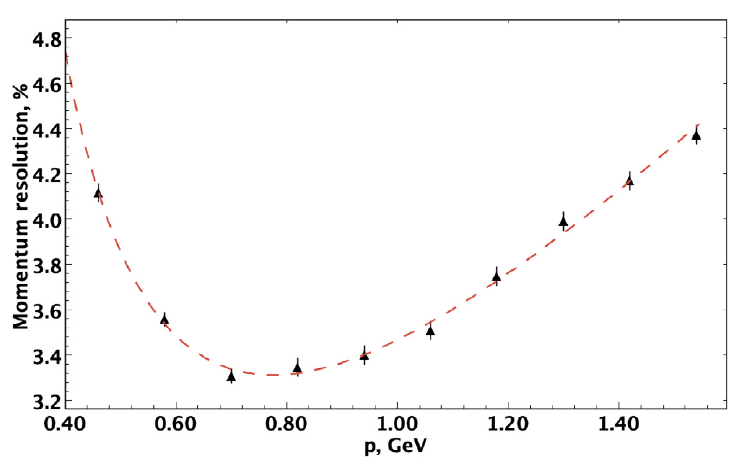
\includegraphics[width=\linewidth]{11experiment/img/23cvt_pres.png}}
        \caption[CVT momentum resolution vs. momentum.]{Momentum resolution vs. momentum of simulated protons in the CVT without background.}
        \label{fig::cvt_pres}
    \end{wrapfigure}

    For both systems, track reconstruction comprises algorithms for pattern recognition and track fitting. Hit objects, corresponding to the passage of a particle through a particular detector component, require the transformation of an electronic signal into a location of the track’s
    position in the detector subsystem geometry.
    A hit is defined as a detector element represented by a geometric object, for example, a line representing a strip in the central tracker.
    These objects then form the input to the pattern recognition algorithms.

    \begin{figure}[t]
        \centering\frame{
        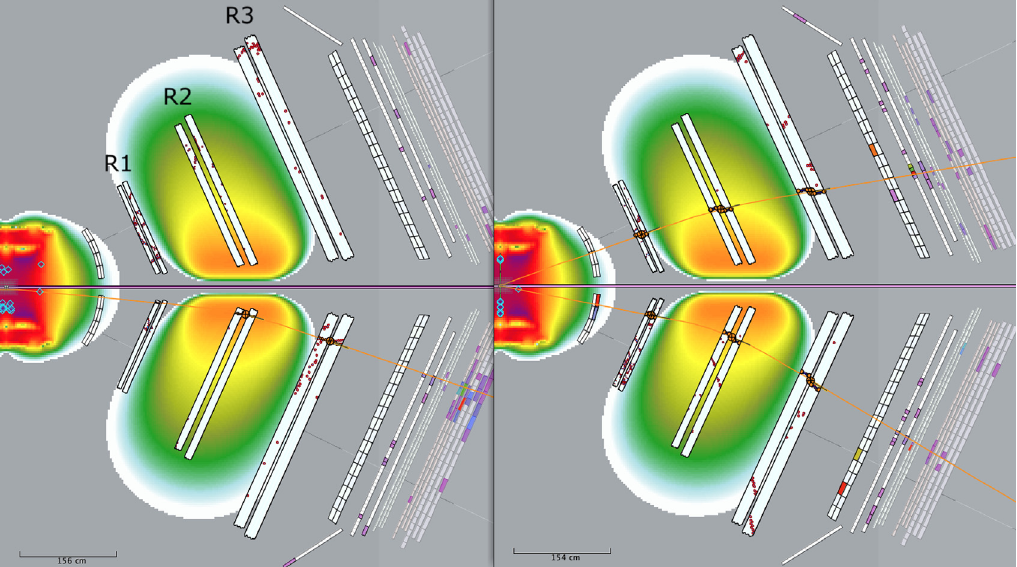
\includegraphics[width=\textwidth]{11experiment/img/23ced_event.png}}
        \caption[Particle going through DC.]{Views from CLAS12 Event Display (ced) of charged particle tracks in the DC showing cut-views to highlight different pairs of sectors of the CLAS12 Forward Detector.
        The coloured detector elements are the registered hits and the orange lines are the result of track reconstruction using the hits in the DC.
        The coloured areas about the detectors represent the regions of magnetic field from the torus and the solenoid.
        In these views the beam is incident from the left and the target is located in the middle of the solenoid (at the left edge of the image).}
        \label{fig::ced_event}
    \end{figure}

    Pattern recognition involves the identification of clusters of hits and the determination of the spatial coordinates and corresponding uncertainties for the hits and clusters.
    At the pattern recognition stage, hits that are consistent with belonging to a trajectory (such as a particle track) are identified.
    This set of hits is then fit to the expected trajectory with their uncertainties, incorporating the knowledge of the detector material and the detailed magnetic field map.
    An illustration of a particle going through the DC can be seen in Figure \ref{fig::ced_event}. 

    % PERFORMANCE.
    The momentum resolutions in the central and forward trackers as a function of momentum are shown in Figures \ref{fig::cvt_pres} and \ref{fig::dc_pres} respectively.
    The distributions are fit with a function of the form $\sqrt{a + bx^2 + c/(1 + d/x^2)}$.
    In both distributions, the worsening of the resolution at low momentum is due to multiple scattering effects.
    The resolution also worsens as a function of momentum after a minimum is reached due to poorer track curvature resolution.

    \begin{wrapfigure}{r}{0.50\textwidth}
        \centering\frame{
        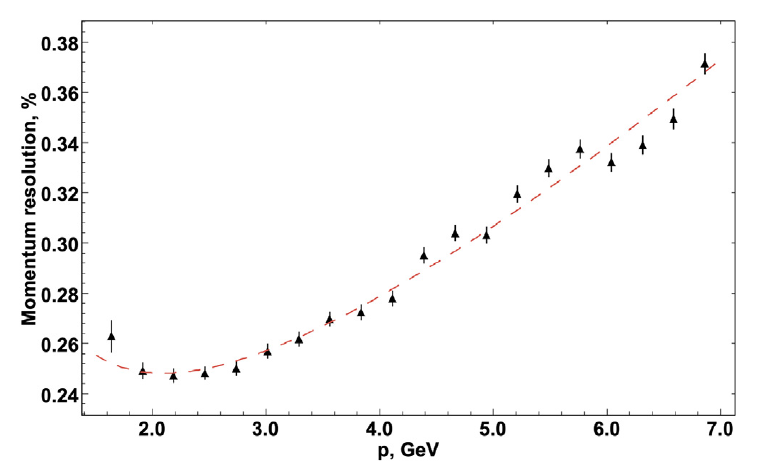
\includegraphics[width=\linewidth]{11experiment/img/23dc_pres.png}}
        \caption[DC momentum resolution vs momentum.]{Momentum resolution vs. momentum in the DC evaluated using pions simulated at $\theta = 15\degree \pm 5\degree$ and at $\phi = 0 \pm 5\degree$ without background.}
        \label{fig::dc_pres}
    \end{wrapfigure}

    For central tracking, an average CVT reconstruction efficiency of $87.3\%$ is obtained from a simulated proton sample with momenta in the range from $0.5$ to $2.5 \text{GeV}$.
    A slight drop of efficiency is observed for tracks with momenta less than $600 \text{MeV}$.
    The higher curvature of small $\text{p}_\perp$ tracks results in an increase in inefficiency due to acceptance effects.
    The dominant source of inefficiency is the gaps between the sensitive volumes for the BMT and the SVT.

    For forward tracking, the momentum resolution in the DC is evaluated using tracks simulated at $\theta = 15\degree \pm 5\degree$ and at $\phi = 0 \pm 5\degree$.
    This is to ensure that most tracks are within the sensitive volume.
    Furthermore, the DC momentum resolution is correlated with the polar angle since the track curvature is determined from the magnetic field intensity, which is higher at lower angles in the torus field.
    These resolutions are obtained from a Monte Carlo sample that does not include out-of-time backgrounds or misalignments of the tracking volumes \cite{ziegler2020}.

\paragraph{Particle Identification}
    % INTRODUCTION.
    The Particle Identification (PID) numbering scheme presented here was introduced by the Particle Data Group (PDG) in 1988 \cite{yost1988}.
    It is intended to aid in interfacing between the various generators, simulators, and analysis packages used in particle physics.
    The system was then revised and adapted in 1998 to allow the systematic inclusion of undiscovered and hypothetical particles \cite{particle1998}.
    The system used in this thesis comes from the most recent version as of the writing of this document, cited from the 2020 Review of Particle Physics by the PDG \cite{particle2020review}.

    The Event Builder (EB) is a service in the reconstruction chain, and performs a series of functions:
    It collects information from the upstream services; correlates information from the sub-detectors into particles; performs a general particle identification scheme; and organises the resulting information into a standardised, persistent data bank structure.
    The service is run twice with identical algorithms, once using hit-based tracks, and later with time-based tracks.
    As mentioned before, the results of the hit-based EB are used to initialise time-based tracking.

    % FORMING PARTICLES.
    In defining a reconstructed charged particle in CLAS12, the EB assumes that an assignment will be made for each reconstructed track in both the FD and the CD.
    The associated calorimeter, scintillator, and Cherenkov detector responses are then assigned to that particle based on geometric coincidences between the detector responses and the track, with matching criteria corresponding to the resolution of a given detector.
    The geometric matching is based on the DOCA between the track and the response.
    A similar procedure is followed for creating neutral particles, except the seeding is presently with unassociated ECAL for the FD and CND for the CD responses instead of tracks.

    % EVENT START TIME.
    A start time is assigned to the entire event and serves as the most precise reference time on which all time-based particle identification relies.
    This is based on the optimal charged particle candidate in the FD with an associated FTOF timing response.
    The EB assigns the start time based on the highest energy electron in the ECAL.
    If there is no electron in the ECAL, it next looks for a positron in the ECAL.
    If there is no lepton, the next track in the priority list is a forward-going positive track (assumed to be a $\pi+$).
    Finally, if there is no forward-going positive track, it looks for a forward-going negative
    track (assumed to be a $\pi-$).
    When looking for $\pi+$ or $\pi-$ tracks, only the candidate with the highest momentum in each group is considered.

    A parallel event start time is determined from the FT to facilitate physics analyses and triggers where the primary scattered electron is at very forward angles in the FT.
    In this case, all combinations of charged particles in the FT and the FD are considered.
    The particle in the FT is assumed to be an electron, whereas all hadron mass hypotheses are considered for the FD tracks.
    The combination with the best time coincidence is chosen.
    The timing of the resulting FT electron is then used to assign the start time.
    A correction to the start time is then performed using the RF signal from the accelerator, combined with the reconstructed event vertex position.
    This effectively aligns the event start time to the best measure of the beam-bunch arrival time at the target.
    The uncorrected, measured vertex time of a particle, $t_v$, can be written as
    \begin{equation*}
        t_v = t - \frac{P_L}{\beta c},
    \end{equation*}
    where $t$ is the measured time response (e.g. in a scintillator), $P_L$ is the path length between the primary interaction vertex and that response, and $\beta c$ is the speed of the particle.
    We can then construct a correction to align this time with the closest beam bunch time at the target, using
    \begin{align*}
        \Delta t_{RF} &= t_v + \frac{z_0 - z_v}{c} - t_{RF} - \frac{N}{2f_{FR}}, \\
        \Delta t^\prime_{RF} &= \text{mod}(\Delta t_{RF}, 1/f_{RF}) - \frac{1}{2f_{RF}},
    \end{align*} % TODO. Not all variables are explained? Try to see what they are from reconstruction.
    where $f_{RF}$ is the frequency of the accelerator, either $249.5 \text{MHz}$ or $499 \text{MHz}$, corresponding to $2.004 \text{ns}$ or $4.008 \text{ns}$ bunch spacings, $t_{RF}$ is the measured, calibrated RF time for the event, and $z_0$ is the target center and enters due to its use as a position calibration reference.
    The resulting RF- and vertex-corrected start time for the event is then given as
    \begin{equation*}
        t' = t_v - \Delta t^\prime_{RF}.
    \end{equation*}

    % PARTICLE IDENTIFICATION.
    The next stage is a basic particle identification scheme.
    This is intended to be loose to accommodate a variety of physics analyses, while persisting the necessary information to easily tighten and improve the criteria later.
    For charged particles, first calorimetry and Cherenkov information is used to positively identify $e-/e+$ candidates in the FD.
    If the measured energy deposition is consistent with the expected sampling fraction of the ECAL, and the photoelectron response from the HTCC is consistent with $\beta \sim 1$, the particle is assigned as an $e-$ or $e+$ depending on sign of the curvature of the track from forward tracking with the DCs through the torus magnetic field.

    The remaining charged particles are then assumed to be hadrons and assigned an identity based solely on timing information, where the $p,K,\pi$ candidate giving the smallest time residual is assigned. 
    This time residual is computed from the difference between the measured particle flight time and that computed for a given mass hypothesis.

    \begin{wrapfigure}{r}{0.49\textwidth}
        \centering\frame{
        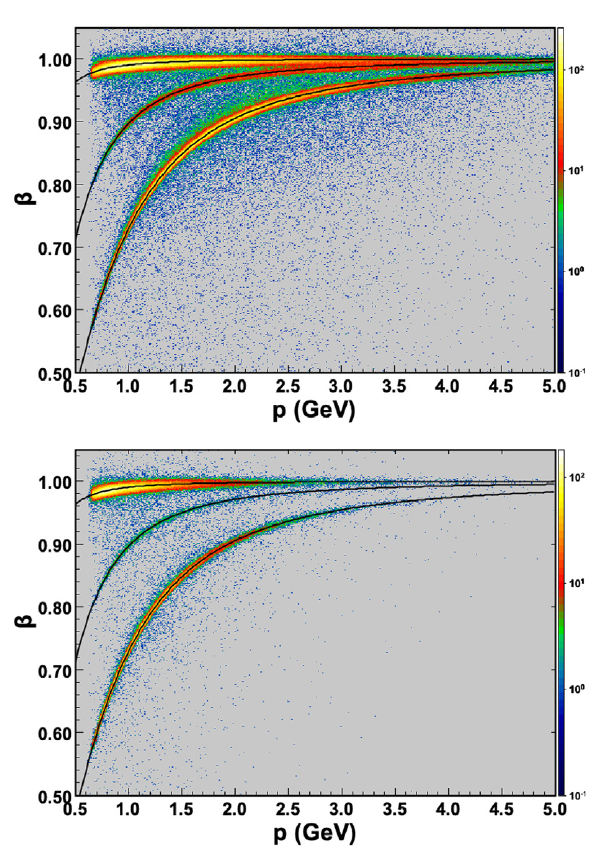
\includegraphics[width=\linewidth]{11experiment/img/23pos_pid.png}}
        \caption[Particle $\beta$ vs. momentum for positively charged tracks.]{Particle $\beta$ vs. momentum from simulation data for positively charged tracks with their start time from an electron in the FD (top plot) or in the FT (bottom plot).}
        \label{fig::pos_pid}
    \end{wrapfigure}

    Figure \ref{fig::pos_pid} shows reconstructed $\beta$ vs. momentum distributions from beam data for forward-going positively charged hadrons using information from the FTOF and DC subsystems, where the electron is reconstructed either in the FD (top) or in the FT (bottom).
    The computed curves for the different mass hypotheses are overlaid.

    Identification of neutral particles assumes only neutrons and photons, differentiated only by timing and topological information.
    For the FD this is based on the ECAL, while for the CD it is based on the CND, and their reconstructed cluster positions are used to compute the particle travel path from the event vertex, assuming a straight-line trajectory.
    If the resulting measured $\beta$ is close to $1$, the particle is assigned as a photon, otherwise it is assigned as a neutron.
    For photons in the FD, the momentum is determined from its deposited energy and ECAL sampling fraction \cite{asryan2020}. % TODO. READ UP ON THIS FOR ANALYSIS WORK.
    For neutrons, the momentum is assigned based on the measured $\beta$, assuming the neutron mass.
    Figure \ref{fig::n_gamma} shows an example of $\beta$ reconstructed for neutrals in the FD showing separation of photons and neutrons.

    \begin{wrapfigure}{r}{0.50\textwidth}
        \centering\frame{
        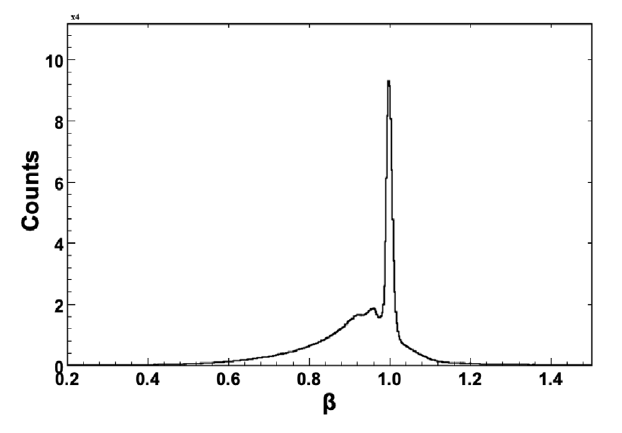
\includegraphics[width=\linewidth]{11experiment/img/23n_gamma.png}}
        \caption[$\beta$ distribution of neutrals.]{$\beta$ distribution for neutral particles as measured by the ECAL from simulation data, showing a sharp peak at $\beta = 1$ from photons and a broader, slower distribution from neutrons.
        }
        \label{fig::n_gamma}
    \end{wrapfigure}

    % PARTICLE IDENTIFICATION PERFORMANCE.
    A particle identification quality factor in the form of a signed-$\chi^2$, or pull, is assigned based on the individual contributing detector subsystem responses and their resolutions.
    For $e-/e+$ identification the resolution-normalised distance from the expected ECAL sampling fraction is used, while for charged hadrons the resolution normalised time-difference is used.
    The resulting information is organised into standardised output bank structures for physics analysis.
    This includes the particle four-vectors, the associated detector responses, and global event information such as beam RF and helicity information.

    The accuracy of the particle identification algorithm that is currently implemented can be estimated from Monte Carlo simulations where the assigned particle identification can be compared to the true one.
    Table \ref{tab::rpid} shows the particle identification matrix for the FD (left) and CD (right).
    The values are based on simulations of electron-hadron or electron-photon pairs with hadron and photon momenta in the range from $1$ to $2.5 \text{GeV}$ and electron momenta in the range from $1$ to $9 \text{GeV}$.
    The diagonal elements correspond to the cases where the particle is correctly identified and the off-diagonal elements to the cases where the particle is misidentified ~\cite{ziegler2020}.
    % Another measure of the particle identification performance for neutrals is given by the reconstruction of $\pi^0$ decays to two photons.

    \begin{table}
        \caption{Particle identification matrix for the FD (left matrix) and CD (right matrix).
        The FD matrix is based on simulated hadrons and photons with momentum between $1$ and $2.5~\text{GeV}$, and electrons up to $9~\text{GeV}$.
        The CD matrix is based on simulated hadrons with momentum between $0.3$ and $1.1~\text{GeV}$.
        The diagonal elements are correctly identified, while the off-diagonal elements are misidentified.
        Detector inefficiencies are included.}

        \begin{tabularx}{\textwidth}{XXXXXXX|XXXXX}
            \hline
                     & \multicolumn{6}{l}{\textit{FD Truth}} & \multicolumn{5}{l}{\textit{CD Truth}}  \\
            \cline{2-12}
                     & $e$      & $\pi$ & $K$  & $p$  & $n$  & $\gamma$ &       & $\pi$    & $K$  & $p$  & $n$  \\
            \hline
            $e$      & 0.98     &       &      &      &      &          &       &          &      &      &      \\
            $\pi$    &          & 0.93  & 0.10 & 0.00 &      &          & $\pi$ & 0.84     & 0.14 & 0.00 &      \\
            $K$      &          & 0.03  & 0.80 & 0.00 &      &          & $K$   & 0.11     & 0.80 & 0.01 &      \\
            $p$      &          & 0.03  & 0.02 & 0.98 &      &          & $p$   & 0.03     & 0.04 & 0.95 &      \\
            $n$      &          &       &      &      & 0.66 & 0.01     & $n$   &          &      &      & 0.11 \\
            $\gamma$ &          &       &      &      & 0.14 & 0.95     &       &          &      &      &      \\
            \hline
        \end{tabularx}
        \label{tab::rpid}
    \end{table}

